\section{Architecture}

This section formalizes the modular components of X-Spanformer and their interactions within the segmentation pipeline. Each architectural unit is presented with motivation, precise mathematical formulation, and pseudocode where appropriate. We conclude with strategies for integrating outputs into standard transformer encoders, including support for overlapping span interpolation, and a runtime complexity analysis.

X-Spanformer is bootstrapped by a compact BPE vocabulary\footnote{\label{fn:bpe}We initialize tokenization with SentencePiece \cite{kudo2018sentencepiece} or similar to avoid fixed-length subword bias while maintaining fast bootstrapping and ONNX compatibility. This follows principles also found in token-free models such as ByT5 \cite{xue2022byt5} and CANINE \cite{clark2022canine}.} and produces:
\begin{itemize}
  \item A ranked span set \(S = \{(i_k,j_k)\}_{k=1}^K\), with \(1 \le i_k < j_k \le L\).
  \item Span embeddings \(s_{i_k j_k} \in \mathbb{R}^d\).
  \item Soft type distributions \( p^\mathrm{type}_{i_k j_k} \in \Delta^T \), \footnote{Here, \(\Delta^T\) denotes the \(T\)-dimensional probability simplex: vectors of nonnegative weights summing to one}, representing modality types such as natural language, code, identifiers, vision, or audio.
  \item A filtered set \(S' \subseteq S\) based on learned length constraints.
\end{itemize}

Span-level augmentation follows the strategy used in models that embed auxiliary semantic units alongside token streams \cite{joshi2020spanbert, devlin2019bert}. Unlike early segmentation-based models that hard-assign phrasal structure \cite{jackendoff1977xbar}, we treat spans as latent soft units learned through boundary confidence and pooling. All modules are trained jointly with the downstream encoder.

\subsection{Seed Embeddings and Candidate Set}

The segmentation process begins with a sequence of base representations, or seed embeddings, which are intended to provide a minimal yet expressive lexical signal for identifying higher-order linguistic structure. These embeddings, derived from a lightweight subword tokenizer, anchor the span predictor in a sparse but stable input space.\footnote{See \cite{kudo2018sentencepiece, sennrich2016bpe, tay2021charformer} for methods on fast and robust subword encoders.}

Formally, given an input sequence tokenized to \(L\) elements, we define the embedding matrix
\[
  E = [e_1, \dots, e_L] \in \mathbb{R}^{L \times d},
\]
where each \(e_i\) is a token-level embedding, and \(d\) is the model’s dimensionality. This sequence is processed through a contextualizing encoder:
\[
  H = \mathrm{Encoder}(E) \in \mathbb{R}^{L \times d},
\]
yielding contextual representations \(H = [h_1, \dots, h_L]\).\footnote{The encoder may be frozen or fine-tuned and can be lightweight (e.g., convolutional \cite{tay2021charformer}) or transformer-based \cite{devlin2019bert, raffel2020t5}.}

From this, the model constructs a complete candidate set of potential spans:
\[
  C = \{(i,j) \mid 1 \le i < j \le L\}.
\]
This exhaustive enumeration is tractable for short sequences and compatible with global attention filtering, as used in segment-aware transformers \cite{joshi2020spanbert, zach2019segmenter, cao2021codegen}.

Each span candidate corresponds to a contiguous subsequence \([h_i, \dots, h_j]\) and will be considered for inclusion in the predicted segmentation. The next module computes scores for each of these.

\subsection{Span Predictor}

The span predictor computes a scalar confidence score for each candidate span \((i,j)\in C\), reflecting how likely that subsequence is to form a coherent semantic or syntactic unit. Inspired by boundary-based approaches in segmentation-aware models \cite{liu2022learnedsegmentation, joshi2020spanbert}, we model start and end positions independently. This simplification makes inference tractable, allows for efficient parallel scoring, and empirically yields high-quality span proposals across domains.\footnote{This factorized assumption follows successful precedents in span-based QA \cite{lee2016learning} and structured pretraining \cite{joshi2020spanbert}.}

We compute unnormalized logits and normalized distributions over token positions:
\begin{align*}
  \ell^s &= W_s H + b_s, \& p^s &= \softmax(\ell^s), \\
  \ell^e &= W_e H + b_e, \& p^e &= \softmax(\ell^e),
\end{align*}
where \(\ell^s, \ell^e \in \mathbb{R}^{L}\) and \(p^s_i\) denotes the probability of a span beginning at position \(i\), with \(p^e_j\) denoting its end at \(j\).

Each span \((i,j)\) is assigned a confidence score by multiplying its boundary probabilities:
\[
  \mathrm{score}(i,j) = p^s_i \cdot p^e_j.
\]

This outer-product scoring approach has been widely used for efficient span extraction in question answering and entity recognition tasks \cite{lee2016learning, xu2022faster}. It biases selection toward spans with high local boundary salience while preserving diversity through length variation.

We then extract the top-\(K\) scoring candidates:
\[
  S = \TopK\left\{ \mathrm{score}(i,j) \mid (i,j) \in C \right\}.
\]

\begin{proposition}[Top-\(K\) Marginal Likelihood]
Let \( p^s \in \Delta^L \) and \( p^e \in \Delta^L \) be independent boundary distributions over \(L\) token positions. Define the induced span measure \( P(i,j) = p^s_i \cdot p^e_j \) over the candidate set \( C = \{(i,j) \mid 1 \le i < j \le L\} \). Then, under the independence assumption, the optimal set of \(K\) spans that maximizes the total marginal likelihood is given by:
\[
S = \TopK \left\{ P(i,j) \;\middle|\; (i,j) \in C \right\},
\]
and satisfies:
\[
S = \arg\max_{\substack{S' \subseteq C \\ |S'| = K}} \sum_{(i,j) \in S'} P(i,j).
\]
\end{proposition}

\begin{proof}
By construction, each candidate span \((i,j)\) is assigned an unnormalized confidence score \(P(i,j)\) under the product measure derived from independent start and end distributions. Since \(P(i,j)\) is nonnegative and additive, selecting the top \(K\) values of \(P(i,j)\) maximizes the total likelihood mass over any subset of size \(K\). This corresponds to exact greedy maximization under the monotonic additive objective \( \sum_{(i,j) \in S'} P(i,j) \). The independence assumption ensures that no additional structural constraint or interaction term modifies this score.
\end{proof}

\subsection{Length Estimator}

While the span predictor yields high-confidence candidates based on boundary positions, it lacks an inductive bias toward plausible internal structure—such as the typical width of syntactic, semantic, or modality-specific spans. To address this, we introduce a length estimator: a learned prior over span widths that filters proposals based on predicted span length compatibility.\footnote{This style of predictive regularization is aligned with latent structure filtering techniques in segmentation-aware pretraining \cite{liu2022learnedsegmentation, liu2022pmlm}, and echoes classic Bayesian constraints in alignment models \cite{kreutzer2021distilling}.}

\medskip
\noindent
For each proposed span \((i,j) \in S\), we define its length:
\[
  \delta = j - i + 1.
\]
We then pool features over the span window:
\[
  v_{ij} = \mathrm{Pool}(H[i{:}j]) \in \mathbb{R}^d,
\]
where \(\mathrm{Pool}(\cdot)\) may be mean pooling, max pooling, or self-attentive aggregation.\footnote{See \cite{liu2018genius, tay2021charformer} for strategies to compress variable-length subsequences using adaptive pooling or dynamic convolutions.}

This representation is passed through a classifier head that outputs a categorical distribution over discretized length bins:
\[
  \ell^\delta = W_\ell v_{ij} + b_\ell,
  \qquad
  p^\delta = \softmax(\ell^\delta),
  \qquad
  \hat\delta = \arg\max p^\delta.
\]
The predicted length \(\hat\delta\) acts as a prior over plausible widths and is compared against the actual span length \(\delta\). We retain only those spans for which the prediction deviates from the ground truth by at most a fixed tolerance:
\[
  S' = \left\{ (i,j) \in S \;\middle|\; |\delta - \hat\delta| \le \tau \right\},
\]
where \(\tau \geq 0\) is a hyperparameter governing flexibility. This length-aware filtering mechanism discourages degenerate, overly short, or overly long span hypotheses, and has been shown to improve accuracy in both text segmentation and vision attention tasks \cite{cheng2021masked, vinyals2015pointer, zach2019segmenter}.

\begin{proposition}[Span Count Upper Bound]
Assume that all gold spans satisfy \(\delta \in [\delta_{\min}, \delta_{\max}]\), and let the tolerance satisfy \(\tau < \delta_{\max} - \delta_{\min}\). Then the number of retained spans satisfies:
\[
  |S'| = \mathcal{O}\left(L \cdot (2\tau + 1)\right).
\]
\end{proposition}

\begin{proof}
Fix a start index \(i\). For each predicted length \(\hat\delta\), the end index must satisfy:
\[
j \in \left[\hat\delta + i - \tau - 1,\; \hat\delta + i + \tau - 1\right],
\]
i.e., a window of size \((2\tau + 1)\). For each of the \(L\) start positions, at most \((2\tau + 1)\) spans can fall within the allowed deviation from \(\hat\delta\), yielding the stated linear bound.
\end{proof}

This procedure constrains the spatial budget of the model, enabling sub-quadratic proposal filtering and tractable decoding over long-form sequences. It also reflects cognitively grounded priors on span regularity and compositional unit length \cite{jackendoff1977xbar, kreutzer2021distilling}.

\subsection{Modality Typing}

Spans in source sequences often originate from heterogeneous subdomains—such as natural language, programming syntax, structured identifiers, numeric expressions, or markup. Accurate identification of a span’s modality enables the model to apply domain-specialized logic (e.g., routing to type-specific heads, enforcing syntax-aware constraints, or improving retrieval and alignment).\footnote{See \cite{lin2021codemix, gupta2022molt} for techniques that use token- or span-level typing to improve generative fluency and interpretability in mixed-modality environments.}

To this end, we introduce a shallow classification head that predicts a probability distribution over \(T\) predefined modalities for each span. Let \(v_{ij} \in \mathbb{R}^d\) be the pooled embedding for span \((i,j)\), produced by the same pooling operator used in the length estimator:
\[
  v_{ij} = \mathrm{Pool}(H[i{:}j]).
\]
We compute logits and a normalized modality distribution:
\[
  \ell^\mathrm{type}_{ij} = W_t v_{ij} + b_t,
  \qquad
  p^\mathrm{type}_{ij} = \softmax(\ell^\mathrm{type}_{ij}).
\]
The vector \(p^\mathrm{type}_{ij} \in \Delta^T\) represents the model’s belief over candidate types, capturing epistemic uncertainty in ambiguous or code-switched contexts \cite{lin2021codemix}. This representation serves three purposes:

\begin{enumerate}
  \item \textbf{Auxiliary Supervision:} When modality annotations are available, a cross-entropy loss between \(p^\mathrm{type}_{ij}\) and gold labels provides an auxiliary training signal. This approach aligns with multitask conditioning frameworks like UnifiedQA \cite{khashabi2020unifiedqa} and improves zero-shot transfer in underrepresented types \cite{gupta2022molt}.

  \item \textbf{Stream Conditioning:} During decoding or cross-attention, type distributions can be used to guide soft routing among specialized decoder blocks or prompt adapters \cite{li2021prefix}, enabling modular reasoning across modalities.

  \item \textbf{Interpretability and Diagnostics:} The modality classifier enhances model transparency by linking segmentation decisions to functional subdomains—especially in token-level mixtures or generated scaffolding tasks.\footnote{This is particularly useful for diagnosing over-segmentation, ambiguous boundaries, or routing errors in compositional data streams \cite{lin2022glaive, tay2021charformer}.}
\end{enumerate}

\subsection{Span Embedding}

Each retained span \((i,j)\in S'\) must be mapped to a fixed-size vector representation suitable for downstream fusion. This embedding is intended to capture both the internal structure and the contextual salience of the span, serving as a condensed representation of its semantic or syntactic role. Effective span encodings have been shown to improve performance in question answering, entity linking, and structured generation tasks \cite{lee2017end, joshi2020spanbert, cheng2020probing}.

We explore two span encoding strategies, inspired by prior work in segment pooling and local contextualization:

\begin{itemize}
  \item \textbf{Mean pooling:} A simple, position-invariant aggregation computed as the average of constituent token vectors:
  \[
    s_{ij} = \frac{1}{j - i + 1} \sum_{k=i}^{j} h_k.
  \]
  This approach is computationally efficient, robust to span length, and has proven effective in prior span-focused architectures such as BiDAF and SpanBERT \cite{joshi2020spanbert, lee2017end}.

  \item \textbf{Local self-attention:} A lightweight transformer block operates over the token subsequence \(H[i{:}j]\), enabling the model to capture internal asymmetries and intra-span dependencies:
  \[
    s_{ij} = \mathrm{SelfAttn}(H[i{:}j]).
  \]
  This mirrors span-centric refinement modules in neural coreference and sequence segmentation models \cite{lee2018higher, tay2021charformer}, offering higher expressivity at moderate computational cost.
\end{itemize}

In practice, both methods can be fused or gated dynamically based on span type or predicted length, enabling flexibility in balancing generalization and expressiveness across heterogeneous spans.

\subsection{Discrete Integration}

In the default architecture, span embeddings are appended to the encoder input to form an augmented composite sequence:
\[
  \tilde{E} = [\, e_1, \dots, e_L,\, s_{i_1j_1}, \dots, s_{i_K j_K} \,] \in \mathbb{R}^{(L+K) \times d}.
\]
This construction allows learned spans to act as soft pseudo-tokens (discrete units with internal semantics derived from upstream modules) which are then jointly contextualized alongside the original input. Similar forms of auxiliary token insertion have been shown to improve performance in span-level tasks, prompt tuning, and cross-modal fusion \cite{guu2020retrieval, li2021prefix, zuo2022rethinking}.

Importantly, standard transformer encoders can process this composite sequence without architectural modification, as the inserted vectors match token dimensionality and participate in multi-head attention identically \cite{devlin2019bert, raffel2020t5, guu2020retrieval}. This approach mirrors the insertion of learned prompt tokens or retrieved vectors into encoder-decoder models without altering core attention mechanics.

However, to prevent positional ambiguity and enforce separation between token and span-originated embeddings, we optionally apply specialized feature encodings (such as segment tags, span-type biases, or learned offsets) to preserve structural grounding \cite{li2021prefix, shaw2018self, xue2022byt5}.
\begin{itemize}
  \item \textbf{Relative offsets:} Span positions can be encoded relative to the input sequence to model anchoring \cite{shaw2018self}.
  \item \textbf{Segment or modality tags:} Type embeddings help disambiguate pseudo-tokens originating from different sources or domains \cite{xue2022byt5, tay2021charformer}.
  \item \textbf{Attention masking:} Optionally restrict cross-token attention during pretraining to reduce information bleed or enforce compositional constraints.
\end{itemize}

While this discrete integration is straightforward in implementation, it serves as a critical interface between low-level segmentation logic and high-level fusion or reasoning stages. Alternative strategies such as early fusion, cross-attention bridging, or gating will be explored in the upcoming sections.

\subsection{Span Interpolation for Overlap Resolution}

To gracefully handle overlapping or redundant spans, X-Spanformer employs a continuous interpolation mechanism over the filtered set \( S' = \{(i_k, j_k)\}_{k=1}^{K'} \). Rather than injecting each span embedding directly, the model computes a relevance-weighted mixture over their representations:
\begin{equation}
  \tilde{s} = \sum_{(i,j) \in S'} \alpha_{ij} \cdot s_{ij}, \label{eq:span_interp}
\end{equation}
where \( s_{ij} \in \mathbb{R}^d \) is the encoded representation for span \((i,j)\), and \( \alpha_{ij} \in [0,1] \) is its normalized attention weight.

\begin{figure}[t]
  \centering
  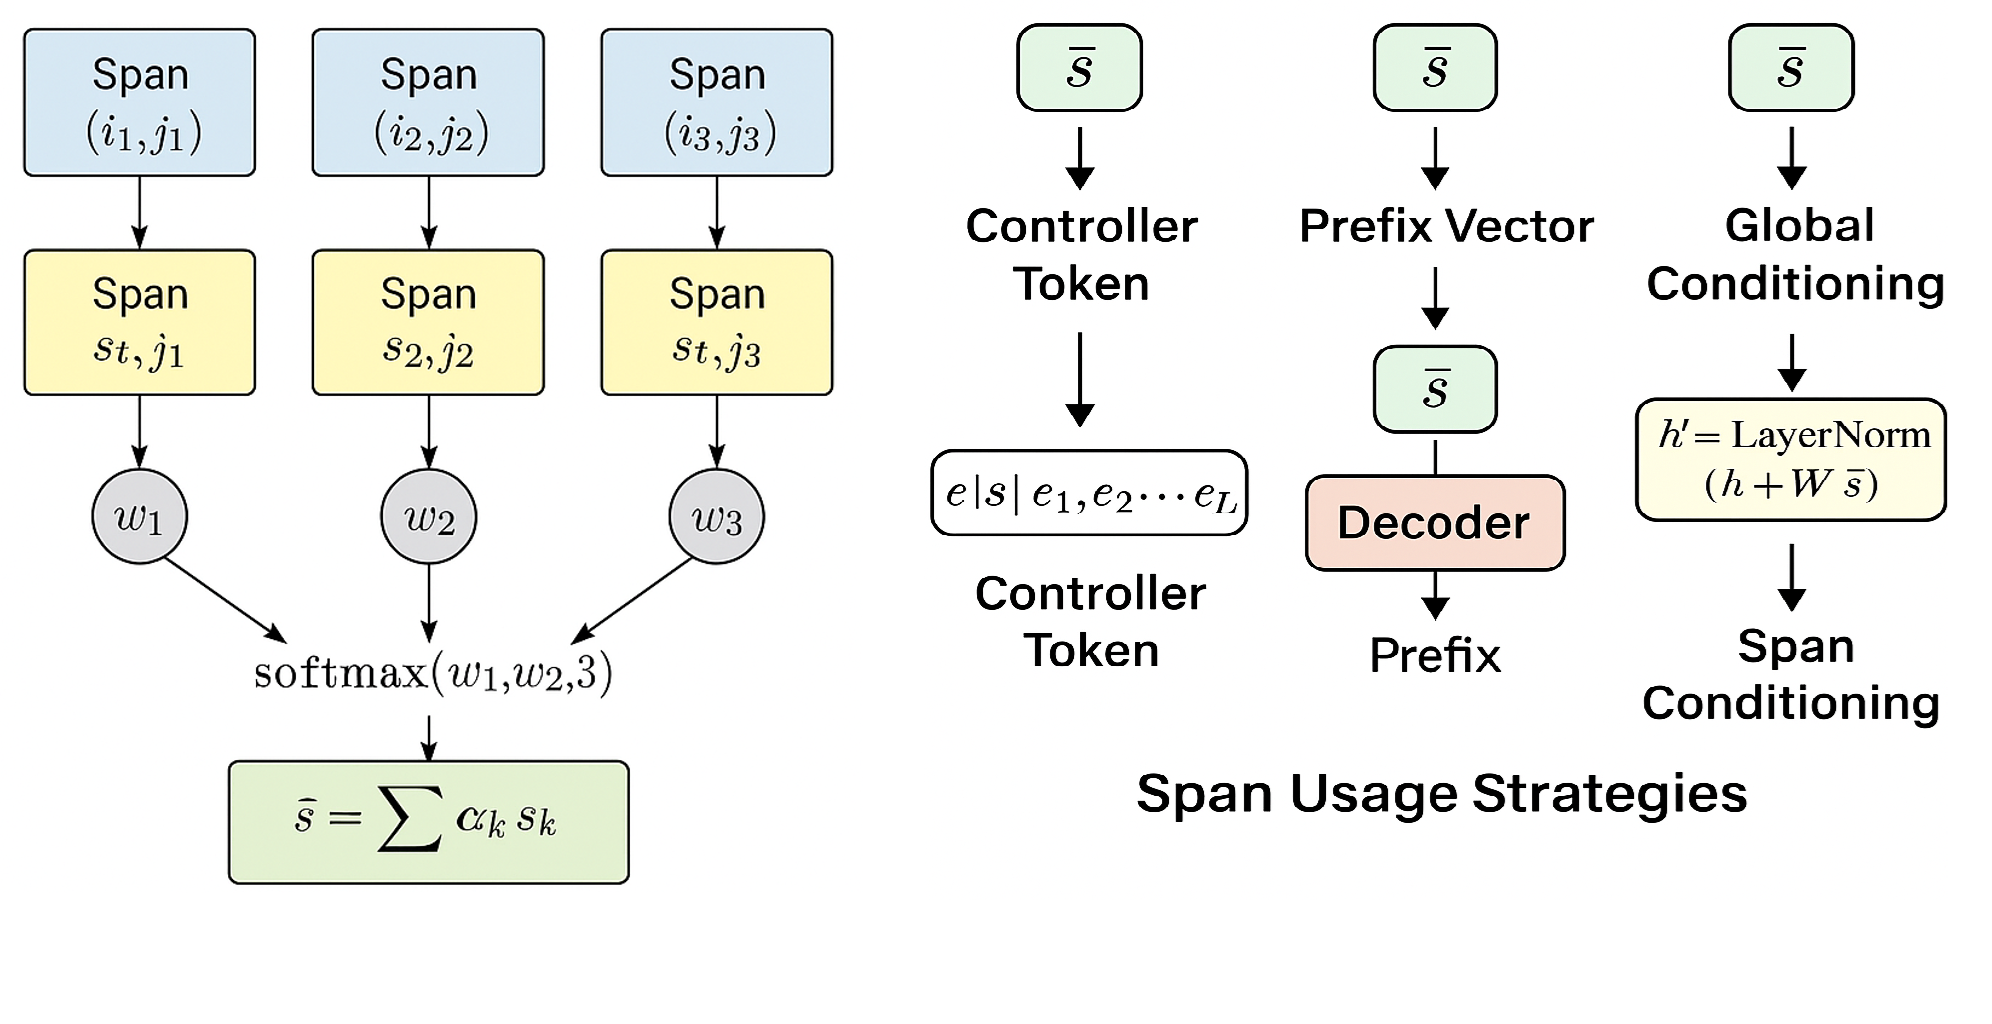
\includegraphics[width=0.95\textwidth]{figures/figure_1.png}
  \caption{Interpolation of overlapping span embeddings and integration strategies. Retained spans are scored by a learned function \( w_{ij} \), normalized via softmax, and fused into a global summary vector \( \tilde{s} \). This vector can be inserted as a controller token, prefix embedding, or conditioning signal for downstream modules.}
  \label{fig:span_interpolation}
\end{figure}

To compute the interpolation weights \( \alpha_{ij} \), each span is assigned a scalar relevance logit:
\begin{equation}
  w_{ij} = f_\mathrm{score}(s_{ij}, \delta_{ij}, p^\mathrm{type}_{ij}, \mathrm{conf}_{ij}), \label{eq:relevance_score}
\end{equation}
which may be a learned function over span length \( \delta_{ij} \), type entropy, boundary confidence, or additional pooled features. A softmax transformation ensures normalization:
\begin{equation}
  \alpha_{ij} = \frac{\exp(w_{ij})}{\sum_{(a,b)\in S'} \exp(w_{ab})}, \label{eq:softmax_weights}
\end{equation}
so that \( \sum_{(i,j)} \alpha_{ij} = 1 \).

The final interpolated vector \( \tilde{s} \) (Equation~\ref{eq:span_interp}) functions as a global span summary. It may be inserted as a controller token \cite{devlin2019bert}, prepended as a prefix vector \cite{li2021prefix}, or concatenated to the sequence input for downstream fusion \cite{zhang2022opt}. Because all operations are differentiable, the interpolation mechanism supports full gradient flow and can be trained jointly with other modules. This method parallels soft memory reading in retrieval-based models \cite{guu2020retrieval, izacard2020distilling}, mixture-based reasoning \cite{arora2022exsum}, and latent fusion in compositional decoding.

\begin{proposition}[Equivariance and Convexity]
Let \( S' \) be any permutation of filtered spans. Then the interpolated vector \( \tilde{s} \) is:
\begin{enumerate}
  \item \emph{Permutation equivariant}: invariant to reordering of spans in \( S' \),
  \item \emph{Differentiable}: gradients propagate through both \( w_{ij} \) and \( s_{ij} \),
  \item \emph{Convex}: \( \tilde{s} \in \mathrm{conv}\{s_{ij} \mid (i,j) \in S'\} \).
\end{enumerate}
\end{proposition}

\begin{proof}
Equivariance follows from the input-order invariance of softmax in Equation~\ref{eq:softmax_weights}. Differentiability holds because both the scoring function and span encodings are differentiable mappings. Convexity arises from expressing \( \tilde{s} \) in Equation~\ref{eq:span_interp} as a convex combination of fixed vectors with weights \( \alpha_{ij} \ge 0 \), summing to 1.
\end{proof}

\subsection{Runtime Complexity}

A key design goal of X-Spanformer is to enhance structural awareness without compromising computational efficiency. To this end, we decompose the end-to-end forward pass into three core stages:

\begin{itemize}
  \item \textbf{Span enumeration and scoring}: generation and scoring of candidate spans from the input sequence;
  \item \textbf{Embedding and selection of top-ranked spans}: pooling span-level representations and selecting a subset for contextual conditioning;
  \item \textbf{Joint contextualization}: applying a standard transformer encoder over the combined sequence of tokens and selected spans.
\end{itemize}

This modular design ensures that added computational cost remains subquadratic for the first two stages, while the dominant quadratic term scales with total input length. Similar hybrid strategies are used in sparse attention transformers \cite{beltagy2020longformer, zaheer2020bigbird} and routing-based models \cite{shazeer2017outrageously, ainslie2023transformers}. The proposition below formalizes the overall runtime cost:

\begin{proposition}[Runtime Bound]
\label{prop:runtime}
Let \(L\) be the input sequence length, \(K\) the number of retained spans, \(w_{\max}\) the maximum span width, and \(d\) the model's hidden dimension. Then the total forward pass runtime of X-Spanformer is:
\[
\mathcal{O}(L w_{\max}) + \mathcal{O}(K d) + \mathcal{O}((L + K)^2).
\]
\end{proposition}

\begin{proof}
The total runtime decomposes into the following:

\textbf{(1) Span enumeration and scoring:} Each of the \(L\) tokens anchors up to \(w_{\max}\) rightward spans. Each span is scored by a parameterized function \(f_\theta(x_{i:j})\), typically an MLP or bilinear form. Hence the cost is:
\[
\mathcal{O}(L w_{\max}).
\]

\textbf{(2) Span encoding and filtering:} After top-\(K\) selection, each span is pooled (e.g., via mean or self-attention) into a vector of dimension \(d\), and scored by span-type and confidence heads. These operations are linear in \(d\), giving:
\[
\mathcal{O}(K d).
\]

\textbf{(3) Joint contextualization:} The final sequence consists of original \(L\) tokens and \(K\) span embeddings, resulting in \((L + K)\) total elements. Processing this sequence using standard transformer self-attention \cite{vaswani2017attention} yields:
\[
\mathcal{O}((L + K)^2 d).
\]
Since \(d\) is fixed during training, we absorb it into the constant, yielding:
\[
\mathcal{O}((L + K)^2).
\]

Adding all components proves the result.
\end{proof}

\begin{figure}[H]
  \centering
  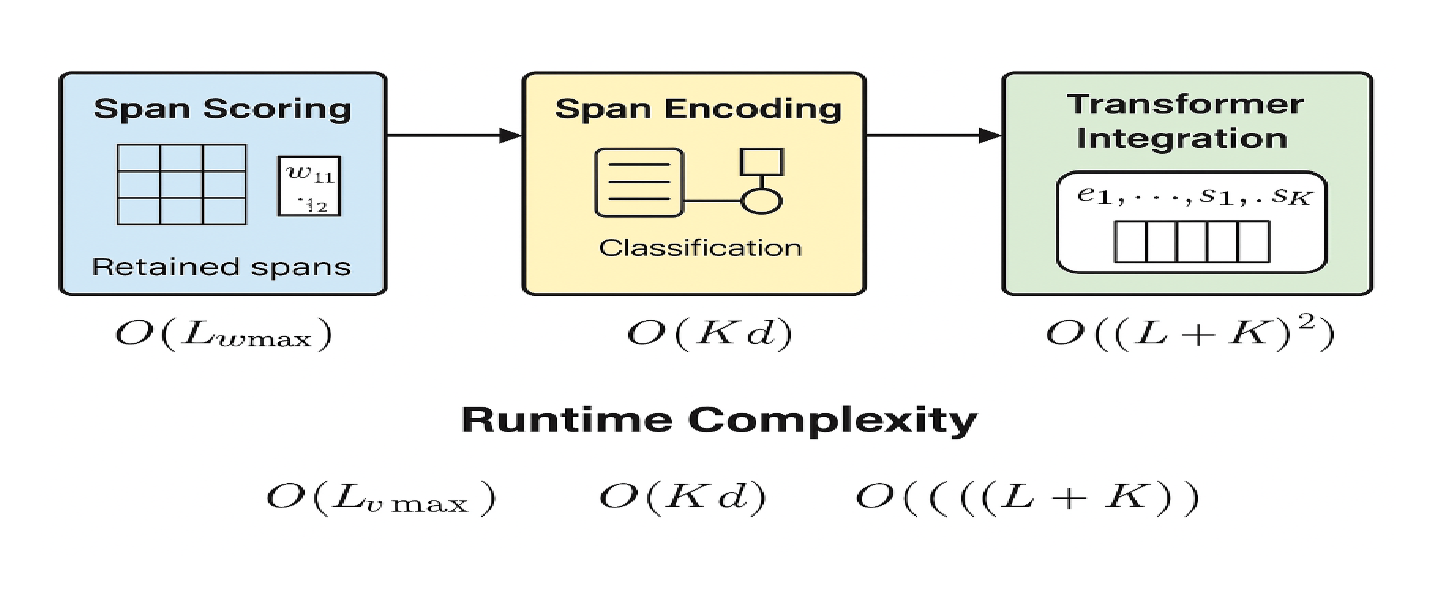
\includegraphics[width=0.92\textwidth]{figures/figure_2.png}
  \caption{Modular runtime decomposition of X-Spanformer's forward pass. Span enumeration and scoring are subquadratic in sequence length \(L\), while span encoding scales linearly with the number of retained spans \(K\). Joint contextualization with self-attention dominates the total cost at \( \mathcal{O}((L + K)^2) \).}
  \label{fig:runtime_decomposition}
\end{figure}